\chapter{آموزش ورژن کنترل}




\section{مقدمه}
ورژن کنترل چیست ؟ و چرا باید به آن اهمیت دهیم ؟ ورژن کنترل یک سیستم ذخیره سازی یک یا چند فایل در طول زمان است \cite{Blischak2016} ورژن کنترل سیستمی است که به توسعه‌دهندگان نرم‌افزار کمک می‌کند تا علاوه بر امکان مشارکت روی پروژه‌های نرم‌افزاری، بتوانند به تاریخچه‌ای از کدهایی که قبلاً نوشته‌اند نیز دست پیدا کنند و به طور کلی اهداف استفاده از سیستم‌های ورژن کنترل را می‌توان در موارد زیر خلاصه نمود:\newline
- فراهم آوردن فرصتی برای توسعه‌دهندگان به منظور کار کردن به صورت هم‌زمان 
- مجزاسازی نسخه‌های توسعه داده شده اختصاصی تک‌تک توسعه‌دهندگان 
- نگهداری تاریخچه‌ای از هر نسخه از هر چیزی که به اشتراک گذاشته شود.\newline
با استفاده از ورژن کنترل شما می توانید ایده های جدید خود را بدون نگرانی آزمایش کنید و در صورت نیاز به ورژن های قبلی برگردید\cite{Chacon2014}. ورژن کنترل سیستمی ضروری برای کار گروهی بر روی یک پروژه نرم افزاری است \cite{DeAlwis2009} . \newline
گیت یک نرم‌افزار کنترل نسخه و از مدل نرم‌افزارهای متن‌باز برای بازنگری کدمنبع توزیع شده و مدیریت منبع کد است که برای دنبال کردن تغییر فایلهای کامپیوتری و دنبال کردن کارهای انجام شده روی آن‌ها توسط افراد مختلف است. که در تمامی سیستم عامل های اصلی توسعه داده شده است \cite{Ram2013} . گیت یک راه قدرتمند برای ردیابی و مقایسه نسخه ها، رفع خطاها، کشف رویکردهای جدید به شیوه ای ساختاری است\cite{spinellis2012git} .\newline
گیت ابتدا برای توسعه لینوکس توسط لینوس تُروالدز به وجود آمد و اکنون پروژه‌های فراوانی از آن الهام گرفته‌اند. هر دایرکتوری کاری در گیت یک مخزن کامل با تاریخچه کامل تغییرها و قابلیت بازنگری آن‌ها است و برای کار با آن نیازی به دسترسی به شبکه یا سرور مرکزی وجود ندارد.\newline
امروزه برنامه نویسی که به گیت مسلط نباشد را عملا برنامه نویس نمیدادند، به عبارت دیگر تسلط به گیت وظیفه ی هر برنامه نویس میباشد. در هرپروژه ای در هر سطحی در دنیا و در هر شرکتی از گیت استفاده میشود حتی شرکت های غیر برنامه نویسی مانند مقاله نویسی ، پایان نامه و هر نوع فایل متنی دیگری میتوان از گیت استفاده نمود؛ مانند همین مقاله که با استفاده از گیت انجام شده است! پس با ما در ادامه این آموزش همراه باشید چون با همین اطلاعات و تمرین آن ها میتوانید آشنایی با گیت را در رزومه خود اضافه کنید.

\newpage

\section{تاریخچه}
همانند بساری از اتفاقات بزرگ زندگی، گیت با یک خرابی و انفجار بزرگ شروع شد!!!
\newline
هسته لینوکس یک پروژه نرم افزاری منبع باز با دامنه نسبتا وسیع است. برای بیشتر عمر تعمیر و نگهداری هسته لینوکس (1991-2002)، تغییرات در نرم افزار به عنوان تکه ها و فایل های آرشیو شده منتقل شد. در سال 2002، پروژه کرنل لینوکس با استفاده از یک DVCS اختصاصی با نام BitKeeper شروع شد.
\newline
در سال 2005، ارتباط بین جامعه که هسته لینوکس و شرکت تجاری که BitKeeper را توسعه داده بود، شکست خورده بود و وضعیت رایگان این ابزار لغو شد. این باعث شد که جامعه توسعه لینوکس (و به ویژه لینوس توروالدز، خالق لینوکس) ابزار خود را بر اساس برخی از درسهایی که در هنگام استفاده از BitKeeper آموخته بودند، توسعه دهند. برخی از اهداف سیستم جدید عبارت بودند از:

سرعت
\newline
طراحی ساده
\newline
پشتیبانی قوی برای توسعه غیر خطی (هزاران شاخه موازی)
\newline
کاملا توزیع شده
\newline
قادر به پردازش پروژه های بزرگ مانند هسته لینوکس موثر (سرعت و اندازه داده ها)
\newline
از زمان تولدش در سال 2005، Git تکامل یافته و بالغ شده است که به راحتی قابل استفاده است و هنوز هم این ویژگی های اولیه را حفظ می کند. این بسیار شگفت انگیز است، بسیار کارآمد است با پروژه های بزرگ، و آن دارای یک سیستم شاخه باور نکردنی برای توسعه غیر خطی است
\newline
\section{کنترل منابع \lr{(Source control)}}

ورژن کنترل های متوعی چون CVN و SVN و bazaar و غیره موجودند اما پدر تمام این برنامه ها Git است! که در تمام شرکت ها و پروژه ها از شما انتظار میرود گیت را بلد بوده و پروژه های خود را ازین طریق ارائه دهید.
\section{گیت \lr{(Git)}}
در این پژوهش به کارایی گیت و همچنین نحوه اجرای دستورات مختلف آن آشنا خواهید شد.
\subsection{شروع کار با گیت}
برای شروع کار با گیت باید نرم افزار گیت را در سیستم خود نصب نمایید.
سپس با با ساختن یک \lr{git dash} در مسیری که میخواهید پروژه خود را شروع کنید صفحه ای باز میشود و میتوانیم در آن دستورات گیت را اجرا کنیم. برای شروع نیاز به دانستن دو نوع شروع پروژه یا ساخت مخزن داریم:
\begin{figure}[tbh]
	\centering
	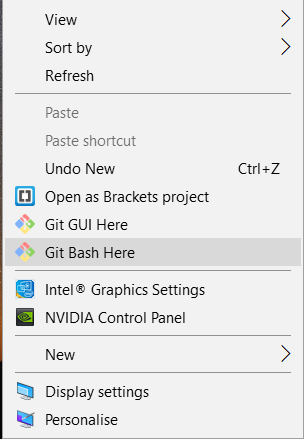
\includegraphics{./Figures/GitBash}
	\caption{ چگونگی ساختن گیت bash  }
	\label{Fig:GitBash}
\end{figure}
\subsubsection{init}
دستور \lr{git init} یک مخزن (repository) جدید ایجاد میکند. این دستور برای تبدیل یک پروژه موجود که ورژنش مشخص نشده به یک مخزن گیت یا ساختن   مخزن جدید خالی مورداستفاده قرار میگیرد. \newline
بقیه دستورات گیت خارج از محدوده ی یک مخزن گیت ساخته شده نیستند. پس بطور معمول این دستور اولین دستور است که شما آن را در یک پروژه جدید اجرا میکنید. \newline
اجرای دستور \lr{git init} یک زیرشاخه دستور \lr{.git } در شاخه ی جاری در حال استفاده میسازد که شامل تمامی متادیتاهایی است که گیت برای ساختن یم مخزن جدید به آن ها نیاز دارد. این متادیتا شامل زیرشاخه ها،مراجع , قالب فایل هااست. \newline
درکنار شاخه \lr{.git } در شاخه ریشه پروژه ، یک پروژه موجود باقی می ماند بدون تغییر میماند.  \newline
به طور پیش فرض، دستور init پیکربندی Git را به مسیر زیرشاخه .git راه اندازی خواهد کرد. مسیر دلخواه را می توانید تغییر دهید و سفارشی کنید اگر دوست دارید آن را در جای دیگر اسفاده کنید. شما می توانید متغیر محدوده  \lr{GIT-DIR } را به یک مسیر سفارشی تنظیم کنید و در ابتدا دستور init فایل های پیکربندی Git را در آنجا راه اندازی خواهد کرد. علاوه بر این شما می توانید یک آرگومان separate-git-dir برای نتیجه ی مشابه منتقل کنید. یک مورد استفاده معمول برای یک زیرگروه جداگانه .git این است که پیکربندی سیستم شما را در پوشه اصلی حفظ کند و پوشه .git را در جای دیگر نگه دارد.
\newline
\begin{figure}[tbh]
	\centering
	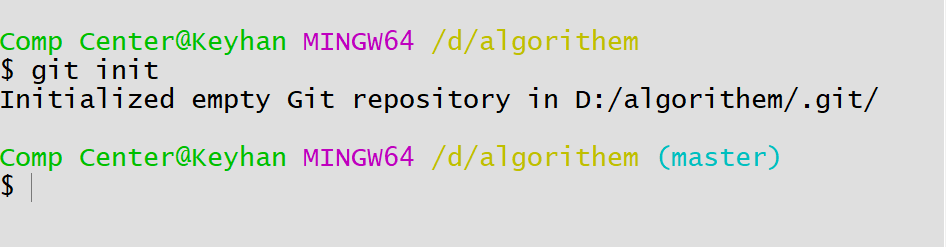
\includegraphics[width=1\textwidth]{./Figures/GitInit}
	\caption{ اعمال دستور init بر روی یک شاخه دلخواه در محیط گیت bash }
	\label{Fig:GitInit}
\end{figure}

\newpage
\subsubsection{clone}
این دستور برای دانلود یک ریپازیتوری موجود در شبکه استفاده میشود. در واقع ما میتوانیم با استفاده از این دستور یک فایل .git موجود در شبکه که میتواند سایت هایی مانند gitlab یا github و یا گیت شرکت شما باشد را در یکی از شاخه های سیستم خودمان داشته باشیم. مانندشکل \ref{Fig:GitClone}    \newline این دستور عینا پروژه را در مسیر منتخب شما کپی میکند، و شما میتوانید آن را تغییر داده و ادامه دهید. \newline گیت کلون تنها یک کپی کاری ساده نیست، بلکه با این دستور شما در واقع یک کپی از تمامی اطلاعاتی که سرور دارد است. تمامی ورژن ها ، تغییرات اعمال شده بر آنها در طول زمان است. \newline در حقیقت، اگر دیسک سرور شما خراب شود، شما اغلب می توانید تقریبا هر یک از کلون ها را بر روی هر سیستمی در شبکه بکار ببندید تا سرور را به حالت ای که در زمان کپی شدن آن بود، بازگردانید.  
\newline
\newline
\begin{figure}[tbh]
	\centering
	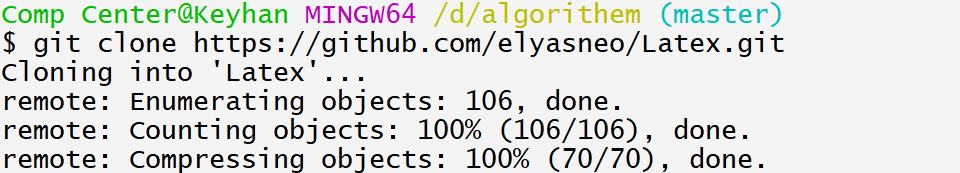
\includegraphics[width=1\textwidth]{./Figures/GitClone}
	\caption{ دانلود روند همین پروژه از گیت لب از پروژه مشترکان   }
	\label{Fig:GitClone}
\end{figure}
\subsection{بررسی و دستیابی}
یکی از محاسن گیت این است که ما میتوانیم در هر لحظه تغیررات ایجاد شده بر روی هر فایل را مشاهده کنیم ! فایل های تغییر یافته را بشناسیم و در کل وضعیتی که داریم را مشاهده کنیم. همینطور میتوانیم به گذشته برویم و به ورژن های مختلف دسترسی داشته باشیم.
این ویژگی بسیار در کار ما با گیت اهمیت دارد زیرا گاها پیش می آید که فرضا در حین انجام یک بخش از کار نیاز به نصب نرم افزار بر یک سیستم یا ایجاد یک باگ شود که نیاز به دسترسی به نسخه های قبلی برای نصب و یا ایراد یابی باشد. 
\subsubsection{status}
دستور گیت status  وضعیت دایرکتوری کار و منطقه پیمایش را نمایش می دهد. این به شما اجازه می دهد ببینید کدام تغییرات مرتب شده اند و کدام فایل ها توسط Git ردیابی نمی شوند. خروجی این دستور شما هیچ اطلاعاتی را نشان نمی دهد برای این کار باید از گیت log استفاده کنید. شکل های را ببینید: \ref{Fig:GitStatus} در این تصویر فایل های قرمز ابتدایی فایل های تغییر یافته و فایل های قسمت دوم فایل های که توسط گیت ردیابی نمیشوند را نمایش میدهد.  
\begin{figure}[tbh]
	\centering
	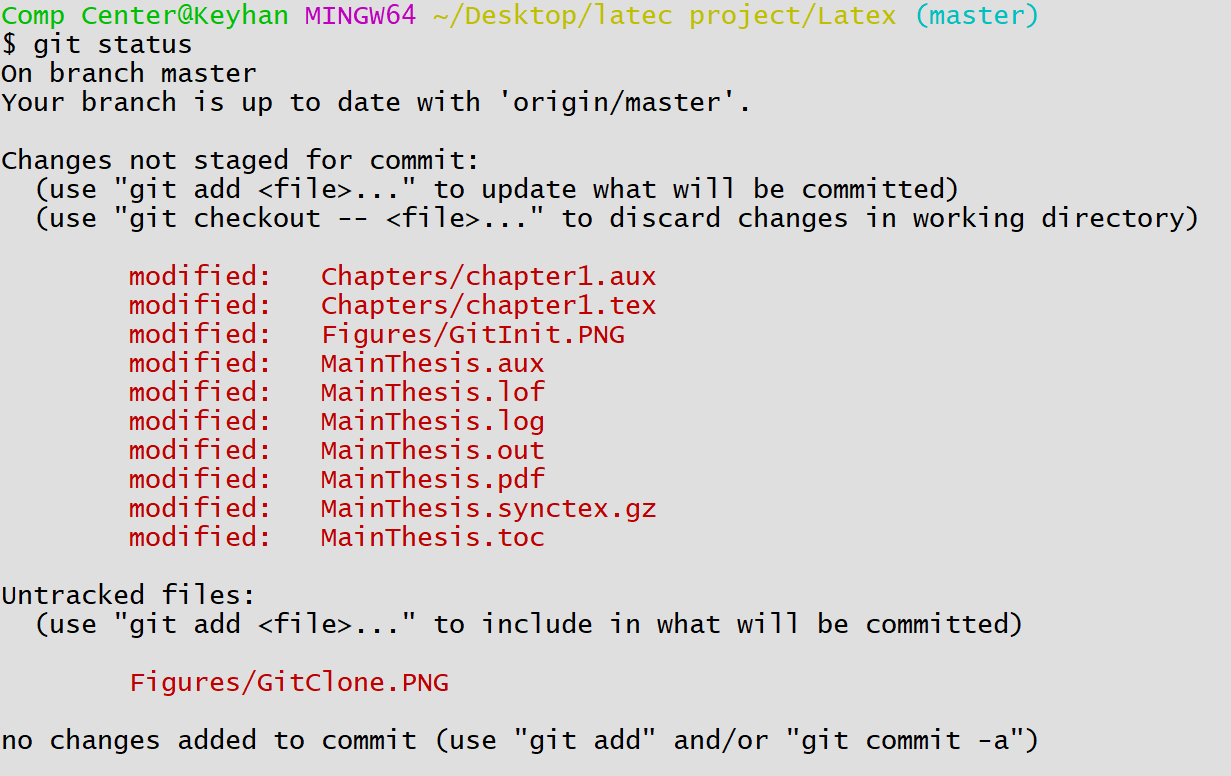
\includegraphics[width=1\textwidth]{./Figures/GitStatus}
	\caption{ گیت استتوس بر روی روند مقاله فعلی بر شاخه .git }
	\label{Fig:GitStatus}
\end{figure}
\newpage
\subsubsection{log}
با اجرای این دستور لیستی از کامیت هایی که تاکنون بر روی شاخه انجام شده است مشاهده میشود، شکل را ببینید: \ref{Fig:GitLog}
\begin{figure}[tbh]
	\centering
	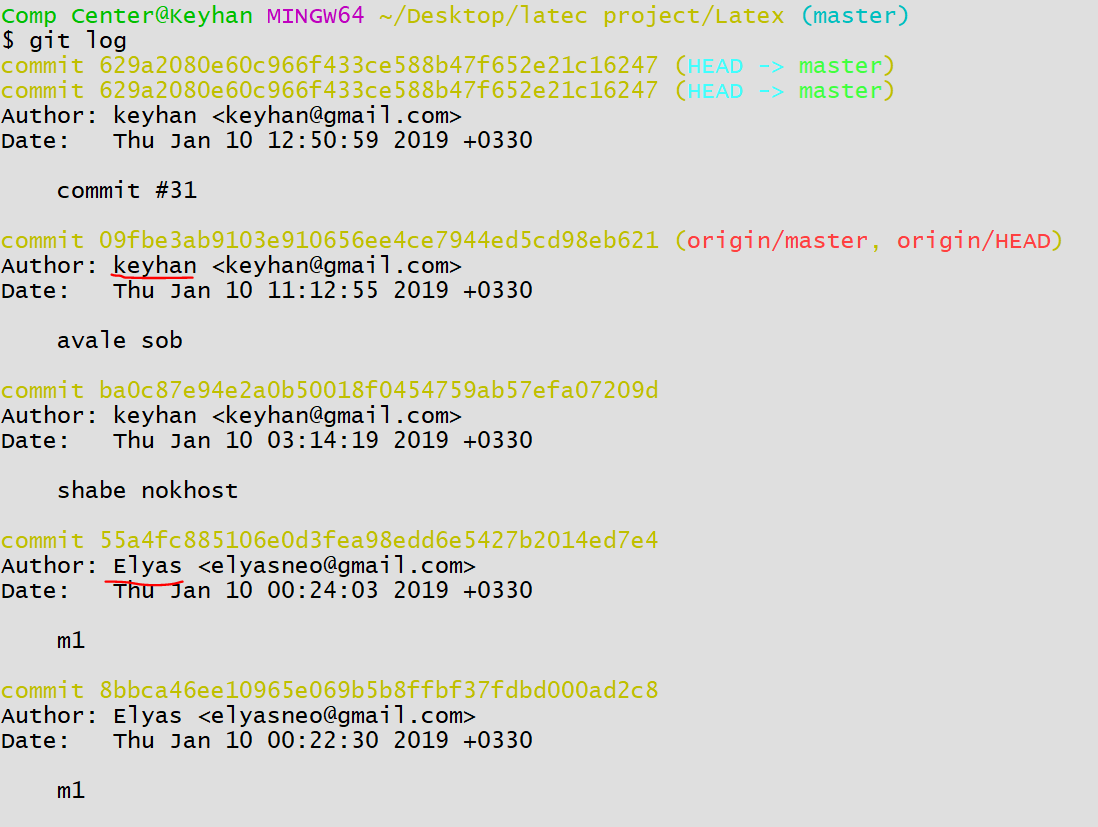
\includegraphics[width=1\textwidth]{./Figures/GitLog}
	\caption{  مشاهده کامیت های انجام شده بر روی مقاله کنونی تا بدینجای کاربا دستور گیت log }
	\label{Fig:GitLog}
\end{figure}
%\subsubsection{diff}
\subsubsection{checkout}
دستور checkout عمل تغییر بین نسخه های مختلف یک موجودیت هدف است. این دستور بر روی سه موجودیت مجزا عمل می کند: فایل ها، commit ها، و شاخه ها. علاوه بر تعریف «checkout»، عبارت «چک کردن» معمولا به معنای اجرای دستور فرمان گیت checkout است. در موضوع لغو تغییرات، ما شاهد چگونگی استفاده از گیت  Checkout برای مشاهده اعمال قدیمی بودیم. اکثر تمرکزاین سند بر عملیات checkout در شاخه ها است.
\newline
چک کردن شاخه ها مشابه چک کردن قرارداد های قدیمی و فایل ها در آن است که دایرکتوری کاری برای مطابقت با شاخه انتخاب شده به روز می شود؛ با این حال، تغییرات جدید در تاریخ پروژه ذخیره می شود - یعنی یک عملیات فقط خواندنی نیست. \newline
در شکل \ref{Fig:GitCheckout} ابتدا به یک نسخه قدیمی میرویم و بعد در شکل \ref{Fig:GitCheckout2} با دستور بعدی به ورژن فعلی برمیگردیم!
\newline
\begin{figure}[tbh]
	\centering
	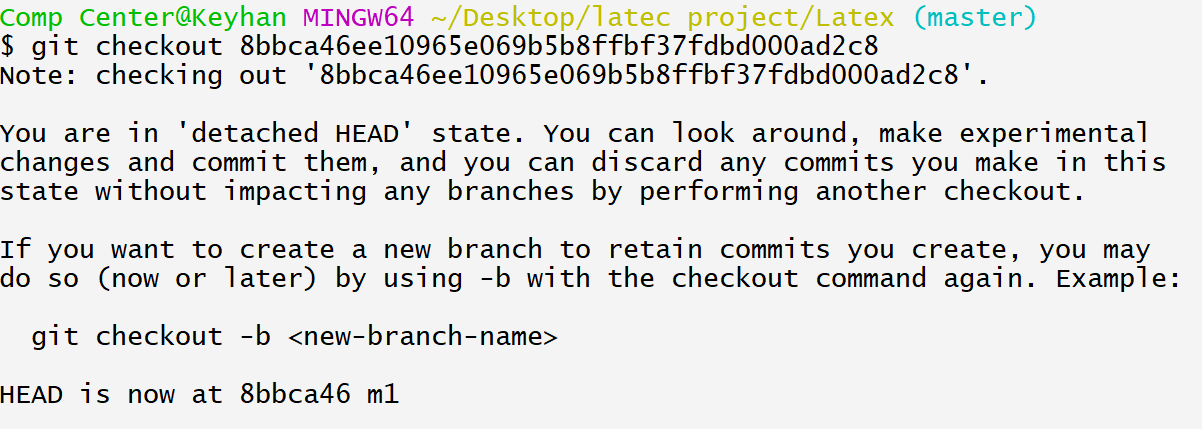
\includegraphics[width=1\textwidth]{./Figures/GitCheckout}
	\caption{ به ورژن های قبلی}
	\label{Fig:GitCheckout}
\end{figure}
\begin{figure}[tbh]
	\centering
	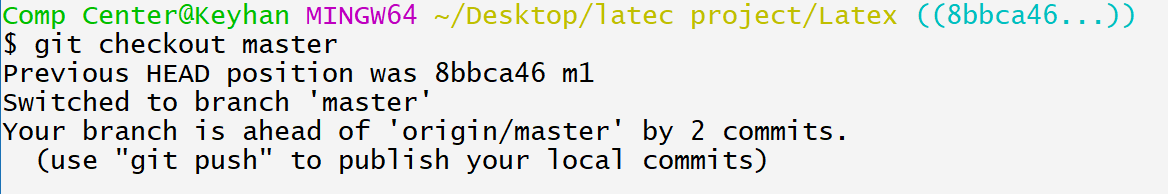
\includegraphics[width=1\textwidth]{./Figures/GitCheckout2}
	\caption{ برگشت به ورژن master }
	\label{Fig:GitCheckout2}
\end{figure}
\subsection{اعمال تغییرات}
پس از تغییر دادن هر فایل اگر از انجام آن تغییر مطمئن هستید میتوانید آن تغییرات را ذخیره کنید. در اینجا روند تغییر هر فایل را با هم یاد میگیریم:
\subsubsection{add}
پس از اعمال تغییر روی هر فایل برای ثبت کردن این تغیررات ابتدا باید آن فایل را در لبه یا همان stage قراردهیم! با این دستور فایل های تغییر یافته در آستانه ی ثبت تغییر قرار میگیرند. \ref{GitAdd}
\begin{figure}[tbh]
	\centering
	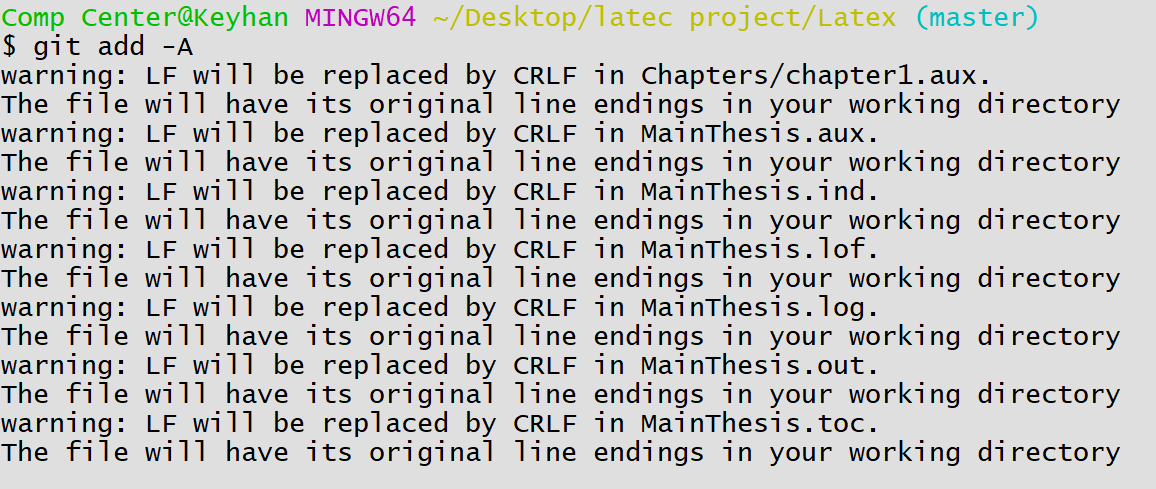
\includegraphics[width=1\textwidth]{./Figures/GitAdd}
	\caption{  مثالی از گیت add   }
	\label{Fig:GitAdd}
\end{figure}
\subsubsection{reset}
دستور ریست برای خالی کردن stage استفاده میشود. هنگامی که ما از یک کامیت پشیمان شدیم قبل از اعمالش میتوانیم با این دستور لبه را خالی کنیم.
\begin{figure}[tbh]
	\centering
	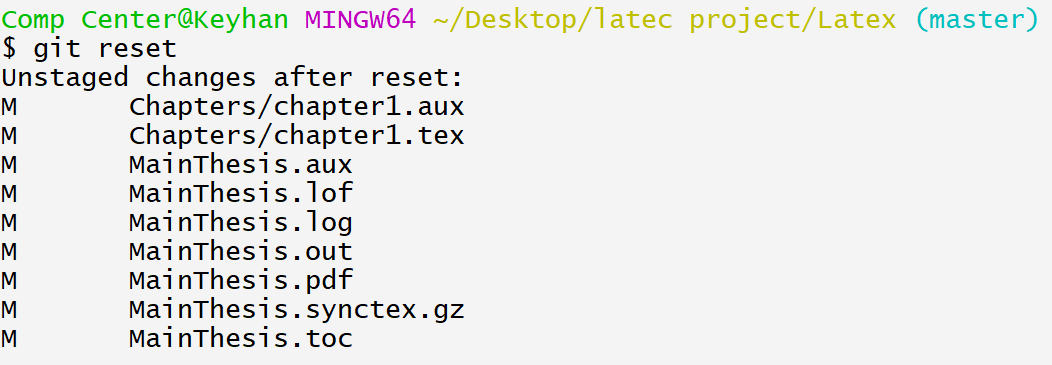
\includegraphics[width=1\textwidth]{./Figures/GitReset}
	\caption{ مثالی از گیت reset }
	\label{Fig:GitReset}
\end{figure}
\subsubsection{commit}
دستور commit محتویات فعلی فهرست لبه را در یک index جدید ذخیره می کند به همراه یک پیام   توصیف تغییرات که توسط کاربر وارد میشود.
\begin{figure}[tbh]
	\centering
	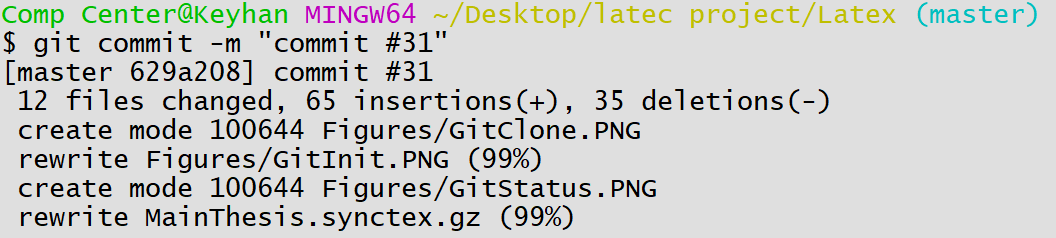
\includegraphics[width=1\textwidth]{./Figures/GitCommit}
	\caption{ مثالی از گیت commit }
	\label{Fig:GitCommit}
\end{figure}
\subsection{توزیع}
در ابتدای خلقت گیت بیان شد که قرار است گیت بر روی سیستم های توزیع شده در دسترس قرار بگیرد که این اتفاق چندی پس از پیدایش آن افتاد. برای فرستادن و دریافت فایل ها به شبکه از دو دستور زیر استفاده میشود؛
\subsubsection{push}
دستور push جهت آپلود فایل جاری بر روی شبکه میباشد ! \newline
بعد از به کارگیری این دستور فایل پروژه با فایل قبلی روی شبکه جایگزین میشود.
\begin{figure}[tbh]
	\centering
	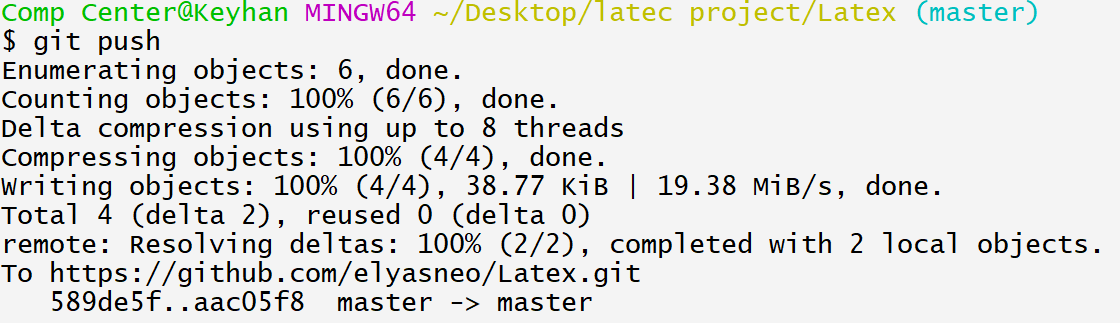
\includegraphics[width=1\textwidth]{./Figures/GitPush}
	\caption{ مثالی از گیت push }
	\label{Fig:GitPush}
\end{figure}
\subsubsection{pull}
دستور pull دقیقا معکوس کار دستور push است. \newline
پس از بکارگیری دستور گیت pull فایل موجود در شبکه جایگزین فایل کنونی میشود و تمام تغییرات و تمام اطلاعات آن به سیستم کاربر می آید.
\begin{figure}[tbh]
	\centering
	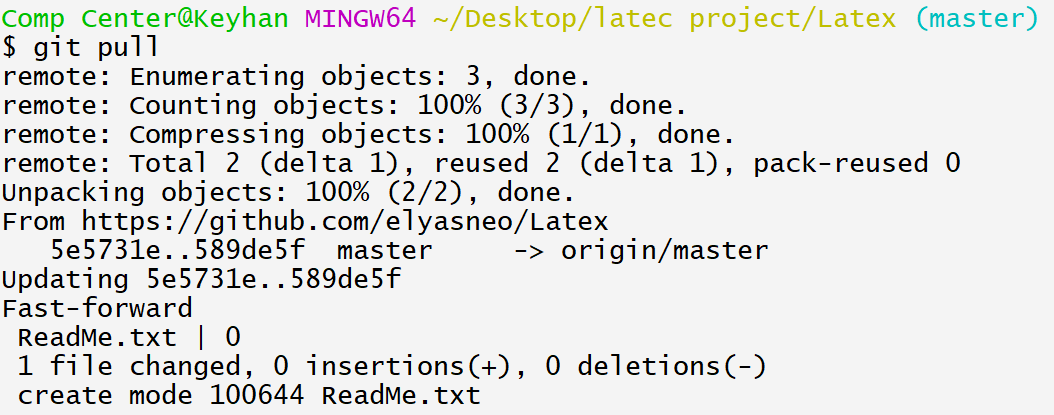
\includegraphics[width=1\textwidth]{./Figures/GitPull}
	\caption{ مثالی از گیت pull }
	\label{Fig:GitPull}
\end{figure}

\subsection{ گسترش }
یکی از قابلیت ها و شاید مهمترین آن ها در گیت امکان ایجاد شاخه در پروژه هاست: یعنی شما میتوانید با استفاده از شاخه سازی یا branching کارهای خود را دسته بندی کنید و هر قایلیت پروژه را بصورت جداگانه انجام دهید! قابلیت های جدید را اضفه کنید یا نسخه هارا مدیریت کنید. \newline
با استفاده از شاخه ها میشود کارهارا بین افراد دخیل در پروژه تقسیم نمود و بدون اینکه لطمه ای به فایل اصلی وارد شود تمام تغییرات را ذخیره نمیود و در آخر نیز با پروژه اصلی ترکیب کرد.
\subsubsection{branch}
شاخه بندی یک ویژگی است که در بسیاری از سیستم های مدرن کنترل نسخه موجود است. شاخه گیری در دیگر VCS ها می تواند عملیات گران در هر زمان و فضای دیسک باشد. در Git، شاخه ها بخشی از روند توسعه روزمره شما هستند. شاخه های Git به طور موثری اشاره گر به عکس فوری تغییرات شما هستند. وقتی میخواهید یک ویژگی جدید اضافه کنید یا یک اشکال را رفع کنید، مهم نیست که چقدر بزرگ یا کوچک است، شاخه جدیدی را برای تغییر دادن تغییرات خود ایجاد می کنید. این باعث می شود که کد ناپایدار به پایه اصلی اصلی ادغام شود و این به شما امکان می دهد تا تاریخ آینده خود را قبل از ادغام آن در شاخه اصلی پاک کنید.
\newline
پیاده سازی پشت شاخه های Git بسیار سبک تر از سایر مدل های سیستم کنترل نسخه است. به جای کپی کردن پرونده ها از دایرکتوری به دایرکتوری، Git یک شاخه را به عنوان یک مرجع به یک مرتبه ذخیره می کند. به این معنا، یک شاخه نشان دهنده نوک یک سری از مرتکبین است - این یک ظرف برای انجام نیست. تاریخچه یک شاخه از طریق روابط متعهد استخراج می شود.
\newline
همانطور که خواندید، به یاد داشته باشید که شاخه های Git مانند شاخه های SVN نیستند. درحالیکه شاخه های SVN تنها برای تسخیر تلاش های گاه به گاه در مقیاس بزرگ توسعه می یابند، شاخه های گیت بخشی جدایی ناپذیر از گردش کاری روزمره شما هستند. محتوای زیر در معماری شاخه داخلی GIT گسترش می یابد.
\subsubsection{merge}
ادغام کردن راه Git برای قرار دادن تاریخچه شاخه دار با هم است. دستور ادغام git اجازه می دهد تا خطوط مستقل توسعه ایجاد شده توسط شاخه git را بسازید و آنها را در یک شاخه واحد ادغام کنید.
\newline
توجه داشته باشید که تمام دستورات زیر ارائه شده به شاخه فعلی ادغام می شوند. شاخه فعلی برای انعکاس ادغام به روز می شود، اما شاخه هدف کاملا تحت تاثیر قرار نخواهد گرفت. باز هم این به این معنی است که ادغام git اغلب در ارتباط با پرداخت git برای انتخاب شاخه جاری و\lr{git branch -d}  برای حذف شاخه منسوخ استفاده می شود.
\newline  \newline \newline
\textbf{در این رشته آموزش با دستور شاخه بندی و گسترش در گیت آشنا خواهید شد:}
\newline
\newline
به عنوان مثال میخواهیم به پروژه یک فایل readMe در شاخه ای جدید اضافه کنیم .
\newline

- شکل \ref{n1} : ساخت شاخه جدید به نام newBranch
\begin{figure}[tbh]
	\centering
	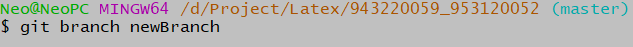
\includegraphics[width=1\textwidth]{./Figures/n1}
	\caption{ }
	\label{n1}
\end{figure}



-شکل \ref{n2} :رفتن از شاخه اصلی به شاخه newBranch
\begin{figure}[tbh]
	\centering
	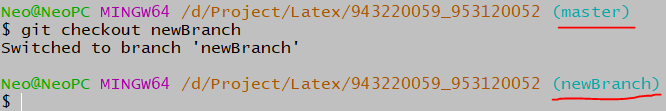
\includegraphics[width=1\textwidth]{./Figures/n2}
	\caption{  }
	\label{n2}
\end{figure}


-شکل \ref{n3} :اضافه کردن فایل readMe در شاخه newBranch و سپس add و commit
\begin{figure}[tbh]
	\centering
	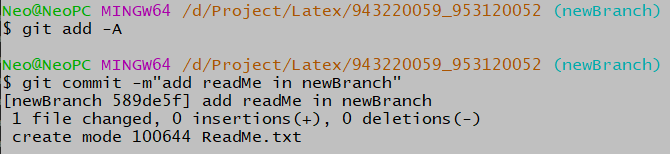
\includegraphics[width=1\textwidth]{./Figures/n3}
	\caption{  }
	\label{n3}
\end{figure}
\newpage


-شکل \ref{n4} :محتویات پوشه پروژه بعد از عملیات گفته شده
\begin{figure}[tbh]
	\centering
	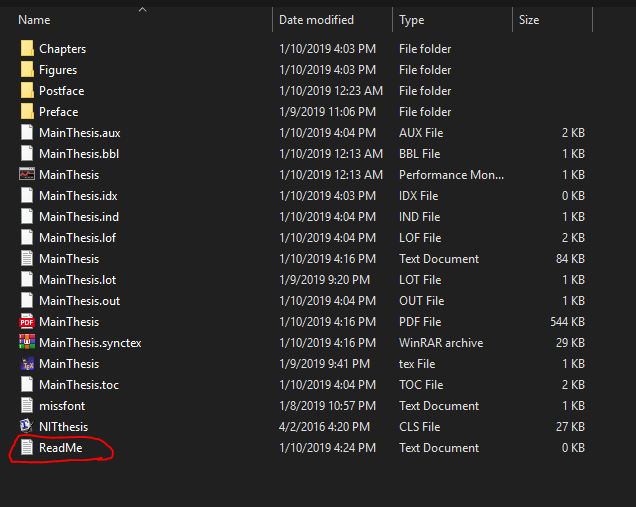
\includegraphics[width=1\textwidth]{./Figures/n4}
	\caption{  }
	\label{n4}
\end{figure}

-شکل \ref{n5} :برگشتن به شاخه اصلی


\begin{figure}[tbh]
	\centering
	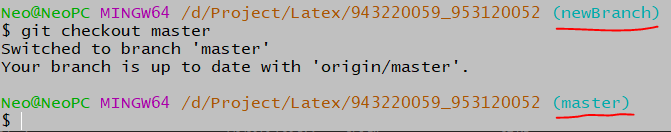
\includegraphics[width=1\textwidth]{./Figures/n6}
	\caption{  }
	\label{n5}
\end{figure}
\newpage

-شکل \ref{n6} :محتویات پوشه پروژه در شاخه اصلی

\begin{figure}[tbh]
	\centering
	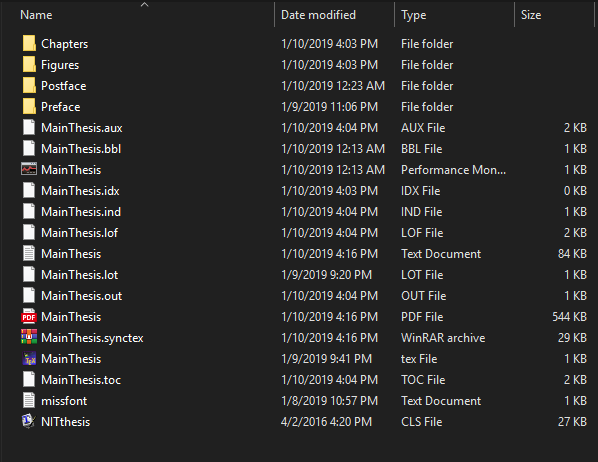
\includegraphics[width=1\textwidth]{./Figures/n7}
	\caption{  }
	\label{n6}
\end{figure}

-شکل \ref{n7} :ترکیب (merge) شاخه اصلی و شاخه newBranch
\begin{figure}[tbh]
	\centering
	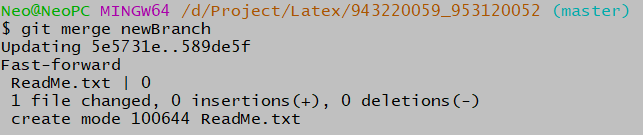
\includegraphics[width=1\textwidth]{./Figures/n8}
	\caption{  }
	\label{n7}
\end{figure}
\newpage

-شکل \ref{n8} :محتویات پوشه پروژه پر شاخه اصلی بعد از ترکیب (merge) 
\begin{figure}[tbh]
	\centering
	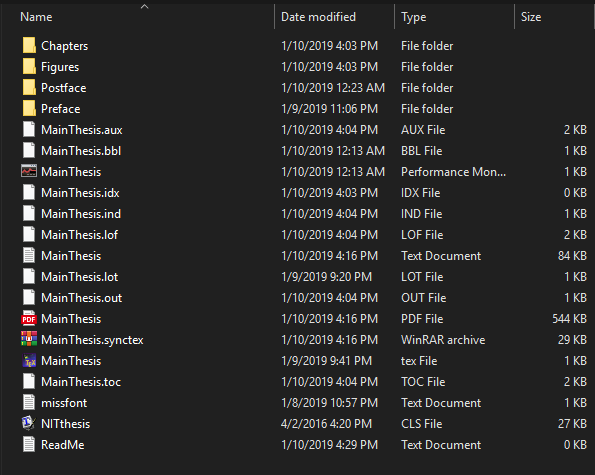
\includegraphics[width=1\textwidth]{./Figures/n9}
	\caption{  }
	\label{n8}
\end{figure}